\chapter[Metodologia]{Metodologia}\label{cap4}

\section{Levantamento Bibliográfico}

A pesquisa bibliográfica foi feita, basicamente, por assunto, por autor e por título. A pesquisa realizada por assunto foi a mais utilizada e termos adequados foram usados para se obter um pesquisa mais efetiva para o entendimento e desenvolvimento do trabalho tais como \textit{audiobooks}, ogg vorbis, livorbisfile, libvorbis, libvorbisenc, compressão de áudio, MDCT, formatos de áudio, WAV, AIFF, MP3, PCM, entre outros. Também foram feitas pesquisas por assunto a respeito de ferramentas necessárias para o desenvolvimento do trabalho tais como formulas latext, player ogg, sox play, dump ogg, convert png to eps, bibtex models example, entre outros. Para a pesquisa feita por autor e título é necessário que já se saiba qual autor ou obra são relevantes para o tema escolhido como, por exemplo, a pesquisa pelo autor Tanenbaum. Levantamento por assunto foi bastante utilizado em pesquisa na internet usando catálogos e mecanismos de busca em sites como o Google Acadêmico \cite{googleacademico}, Google com pesquisa \textit{web} e com filtro para livros, \textit{ACM Digital Library} \cite{acm} e Scielo \cite{scielo}. Ideias e dicas dadas pelo orientador prof. Dr. Edson Júnior deste trabalho foram de suma importância principalmente para uma determinação de ``um ponto de partida''.

Através do levantamento bibliográfica foi possível listar e consolidar citações de trabalhos fundamentais para o tema ou algo similar ao que foi proposto neste trabalho. 

\section{Ferramentas utilizadas}

As ferramentas utilizadas para o desenvolvimento do trabalho são descritas, em poucas palavras, para qual propósito cada uma foi usada e qual a versão utilizada.

Por fornecer ferramentas nativas que ofereceram grande suporte para o desenvolvimento deste trabalho, pelo formato Ogg Vorbis fornecer API de fácil instalação e uso em distribuições Unix e pelo conhecimento prévio do sistema operacional o Ubuntu 14.04 LTS foi adotado para o ambiente de desenvolvimento. O compilador utilizado foi o gcc versão 4.8.2.

O editor de texto utilizado para o desenvolvimento dos códigos fonte em linguagem de programação C foi o Sublime Text 2. Ele foi escolhido por possuir uma interface limpa, por fornecer uma prévia visualização de todo o documento e, principalmente, pelos comandos que ele oferece para facilitar a codificação. Podemos citar como exemplo a troca de linhas sendo possível mover uma linha ou um bloco inteiro de código, cursores múltiplos possibilitando a escrita em diversas parte do código simultaneamente, busca por palavras de mesmo nome e a buscar e substituição de palavras específicas com uma ou múltiplas seleções.

O Latex foi utilizado para desenvolver o trabalho escrito e escolhido por gerar, como saída, um pdf com alta qualidade tipográfica e totalmente formatado. A versão utilizada foi pdfTeX versão 3.1415926-2.5-1.40.14.

Inicialmente foi utilizada a ferramenta hexdump nativa do sistema operacional Unix para mostras os dados binários em hexadecimal com o intenção de facilitar o entedimento do formato de áudio e validar os dados inseridos no formato. Entretanto, a feramenta hexdump foi substituída pela oggz versão 1.1.1. 

A versão v.14.4.1 da ferramenta sox foi utilizada para executar os arquivos de áudio *.ogg com o intuito de verificar se o arquivo não foi corrompido devido as constantes modificações do formato para inserção do pacote de marcação de conteúdo e da inserção dos metadados no cabeçalho de comentários.

\section{Proposta anterior}

Como este trabalho é uma evolução do trabalho realizado por \cite{herbert}, a primeira coisa a ser feita foi entender a sua proposta de trabalho e, para isso, foi feito um estudo em cima de sua monografia. Esta proposta da evolução considerou os problemas levantados e traçou o objetivo de reproduzir o trabalho não originando o mesmo problema e então melhorar o trabalho anterior.

%apenas o software em si, mas também todo o processo de desenvolvimento. Foi levado em consideração os pontos fortes e fracos levantados pelo autor. O autor propôs, inicialmente, o uso de alguns artefatos do RUP e algumas práticas da metodologia ágil. No entanto, como o prazo era curto e a equipe de desenvolvimento era composta por apenas uma pessoa, o processo, de um modo geral, foi ad hoc. Isto explica o fato de ele não ter seguido o que o processo RUP especifica, a saber, a separação das atividades desenvolvidas em Concepção, Elaboração, Construção e Transição. Assim sendo, o processo utilizado também foi ad hoc.

\section{Entendendo o Ogg Vorbis}

O segundo passo foi o estudo de um novo formato: Ogg Vorbis desenvolvido pela fundação Xiph.org. Foi feito um estudo minucioso em cima do documento de especificação do formato Ogg Vorbis para conhecer a sua estrutura e o tipo de suporte que ele oferece. A ferramenta \textit{hexdump} utilizada por \cite{herbert} foi usada como suporte para um melhor entendimento do formato *.ogg. A Figura \ref{hexdump} mostra o resultado da execução do hexdump em um arquivo *.ogg cujo comando é: \$ hexdump -C <file\_name>.

 \begin{figure}[ht]
	\centering
		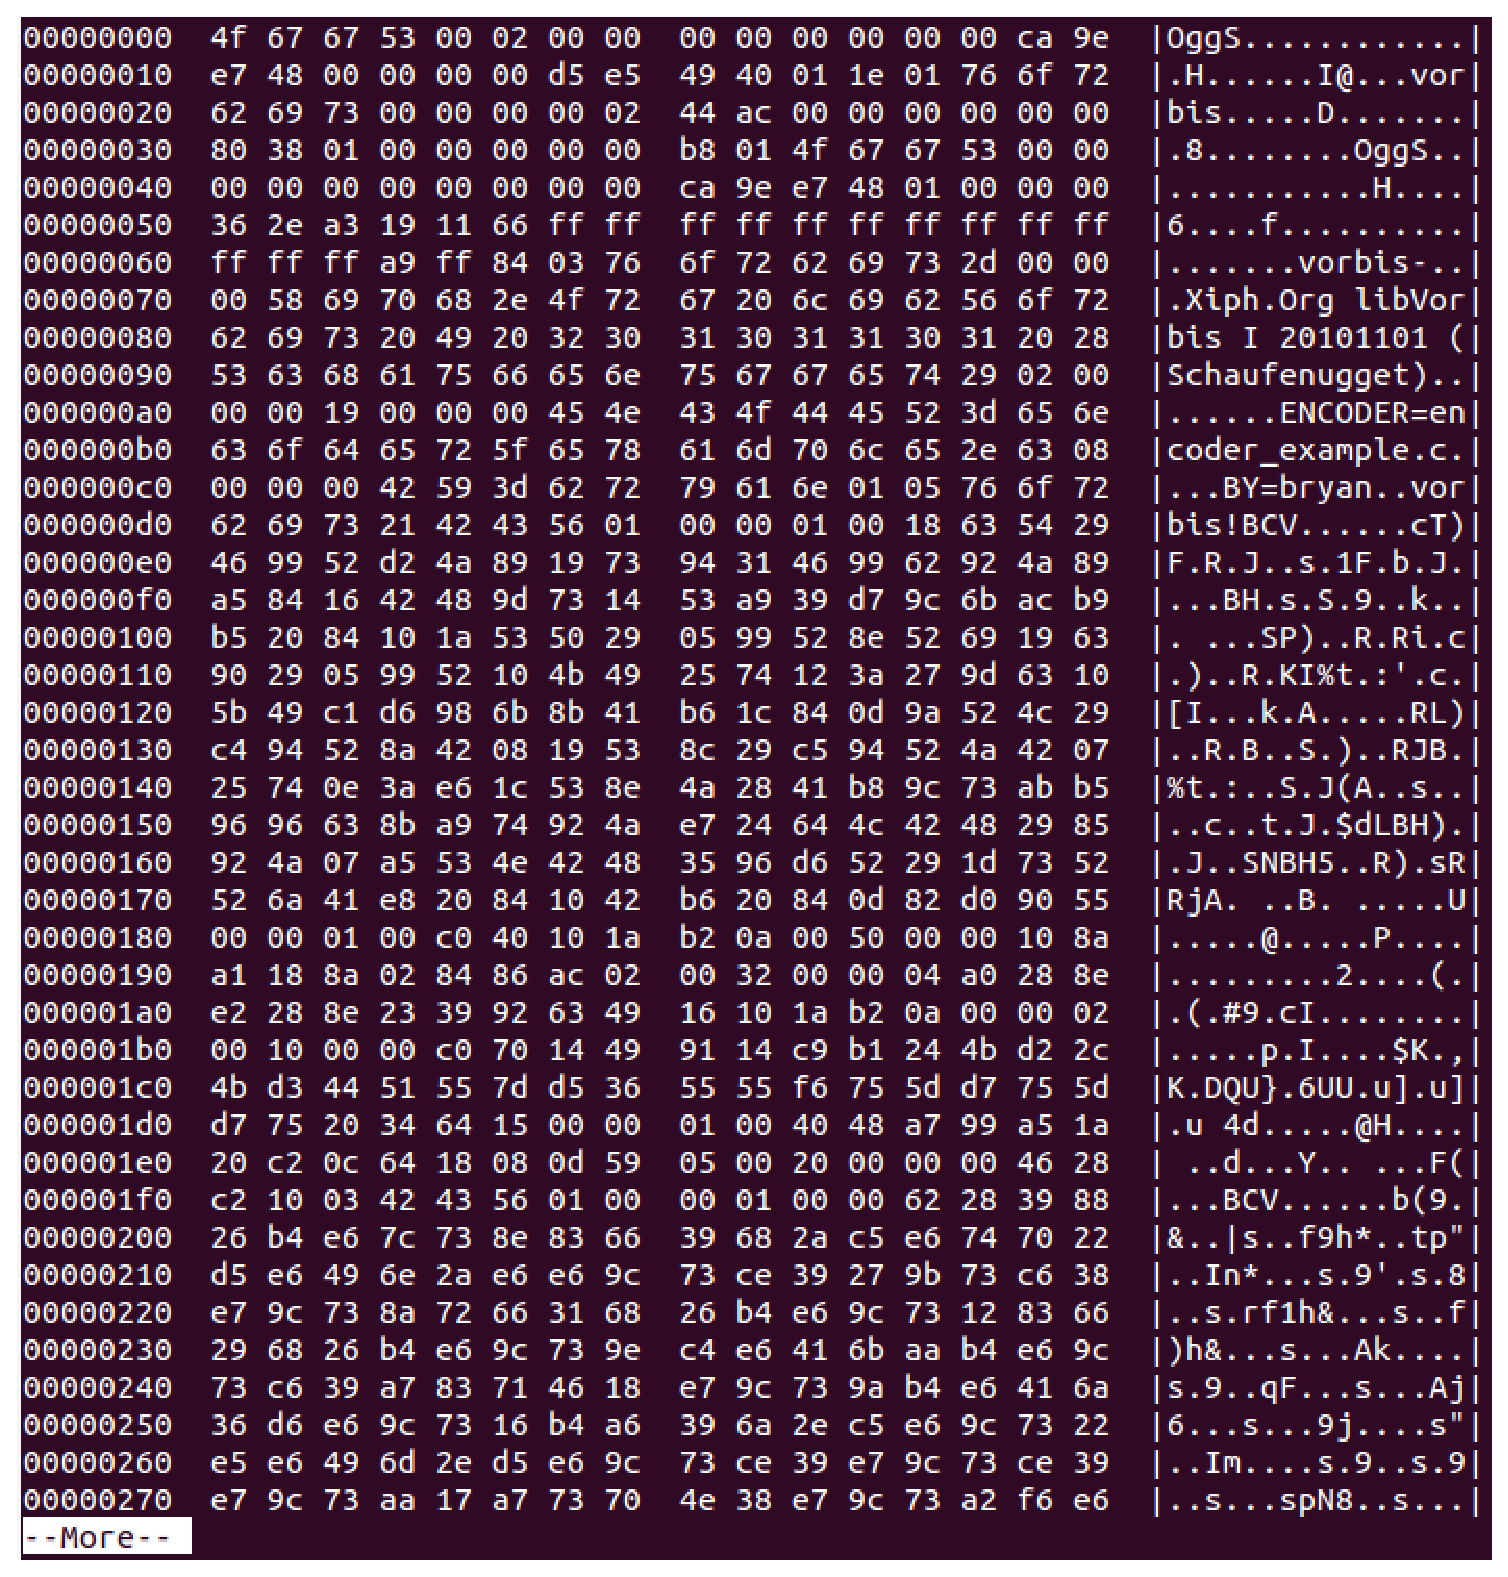
\includegraphics[keepaspectratio=true,scale=0.5]{figuras/hexdump.eps}
	\caption{Execução da ferramenta hexdump.}
	\label{hexdump}
\end{figure}

No entanto, os dados ainda ficaram muito confusos e de difícil interpretação. Após uma pesquisa verificou-se a existência de uma outra ferramenta também nativa no sistema operacional Ubuntu e voltada para os arquivos com extensão *.ogg e possui a mesma finalidade da ferramenta hexdump. A diferença entre elas está na forma com que os dados são apresentados. Podemos verificar na Figura \ref{oggzdump} como o oggz-dump estrutura os dados. O comando para execução da ferramenta é dado no terminal e possui o seguinte formato: \$ oggz-dump <file\_name>.

 \begin{figure}[ht]
	\centering
		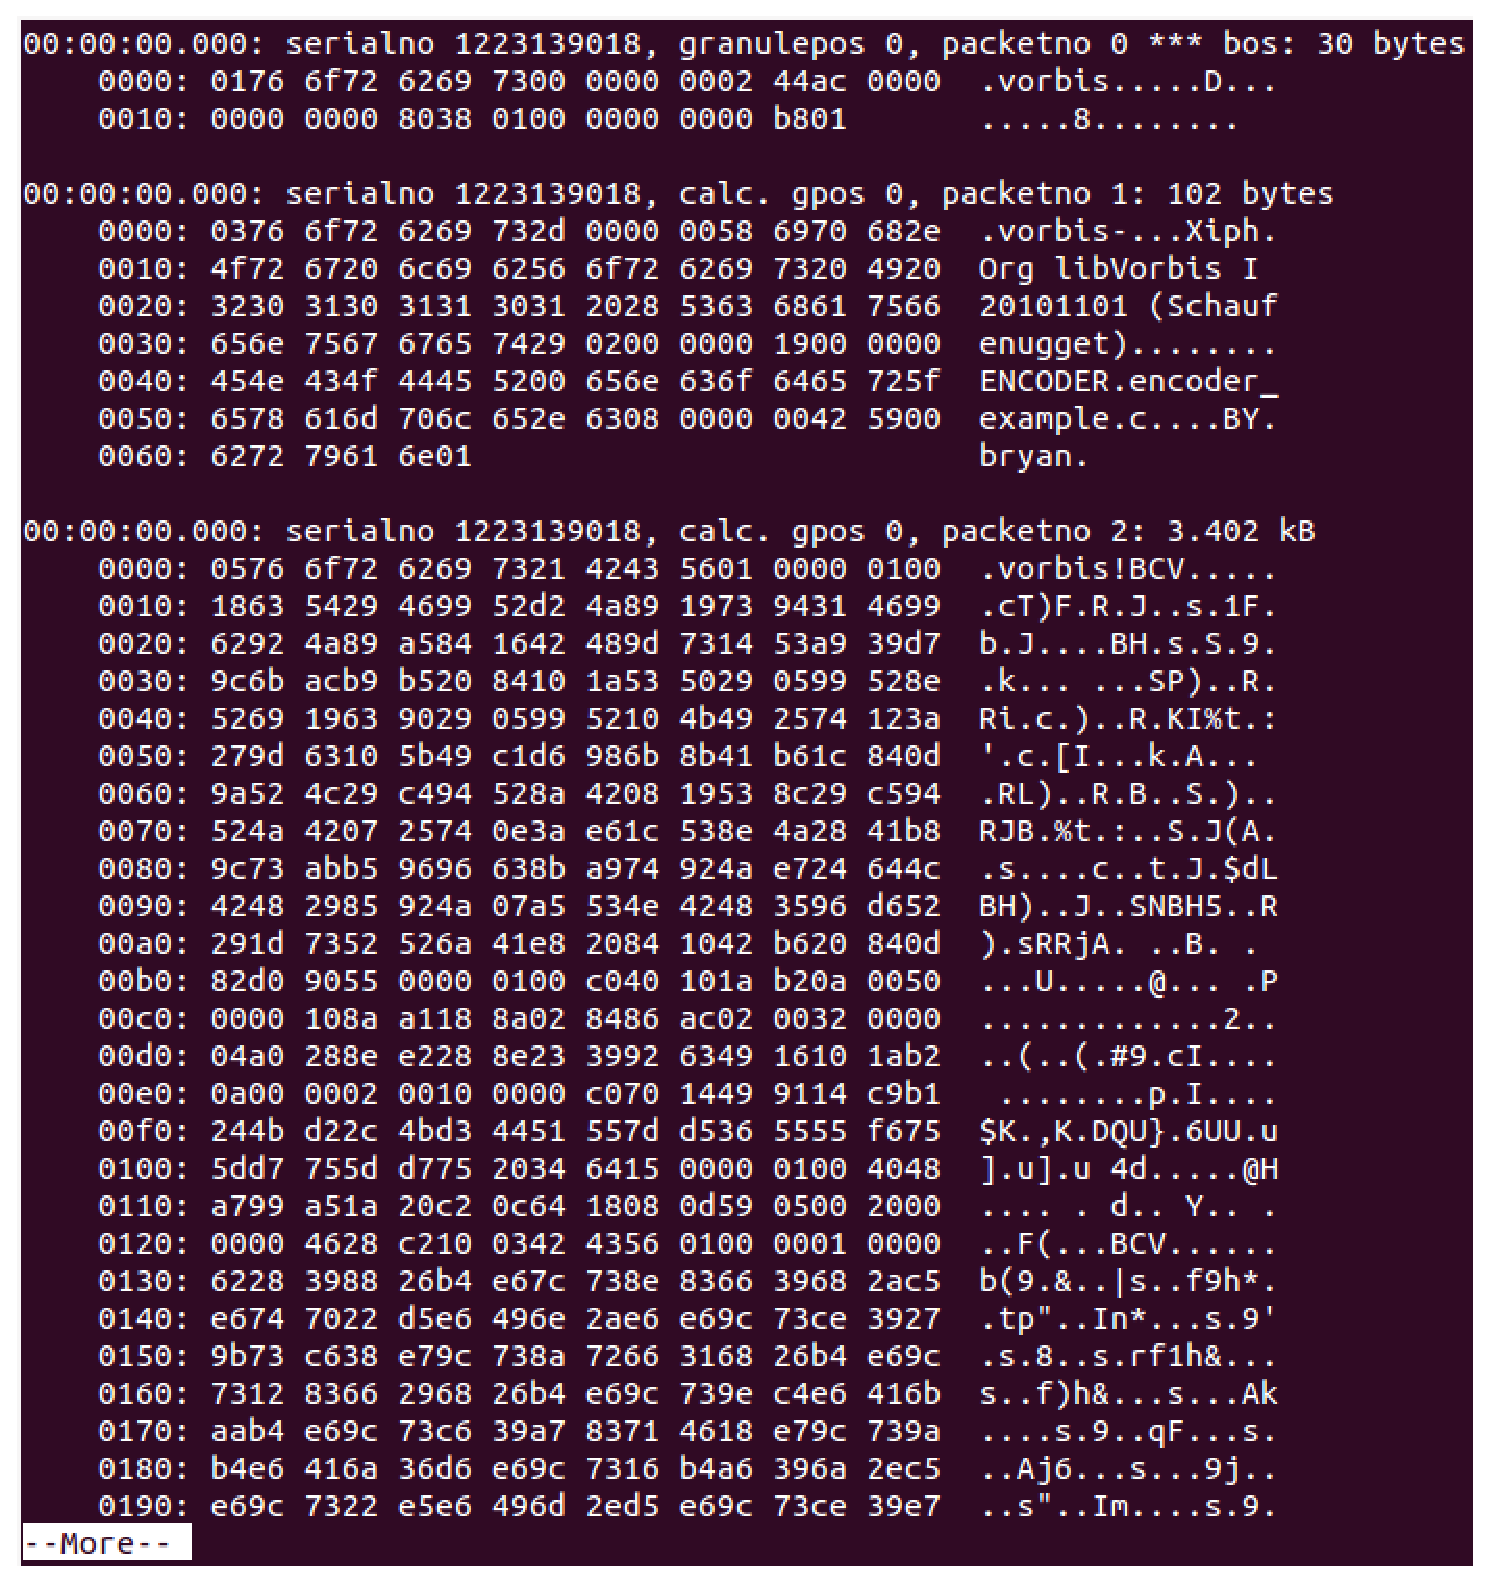
\includegraphics[keepaspectratio=true,scale=0.5]{figuras/oggz-dump.eps}
	\caption{Execução da ferramenta oggz-dump.}
	\label{oggzdump}
\end{figure}

É notável a diferença e a facilidade com que a ferramenta oggz informa sobre os pacotes contidos em um arquivo *.ogg. Após o comando é possível verificar os pacotes separadamente bem como sua informações tais como número do pacote, informações de grânulo, o ``tempo'' em que aquele pacote é lido, o seu tamanho, entre outras informações. Além das informações do pacote também é possível visualizar seu conteúdo e logo percebemos que os pacotes de número 0, 1 e 2 são os pacotes cabeçalhos. A identificação dos pacotes cabeçalhos pode ser percebida pois após o primeiro byte do pacote, os 6 bytes subsequentes contém a string ``vorbis'' onde cada byte representa uma letra.

\section{Construção do codificador}

O estudo e o processo acima foi realizado para entender a estrutura do Ogg Vorbis e onde inserir os metadados e as marcações de conteúdo validando, assim, a possibilidade do uso do formato para a solução do problema. Para dar continuidade no estudo de viabilidade do formato Ogg Vorbis, foi desenvolvido um codificador em linguagem C. Como suporte, foram utilizadas as bibliotecas \textit{libogg}, \textit{libvorbis} e \textit{libvorbisenc}. O \textit{libvorbisenc} é responsável pela codificação. Para compilar o arquivo é necessário utilizar o seguinte comando: 
	
   
   \$ gcc -o <nome\_para\_o\_executável> <código\_fonte> -logg -lvorbis -lvorbisenc


Para garantir que o processo de codificação realmente funcionasse, foi utilizado outro formato no processão de codificação de um formato Ogg Vorbis. O código desenvolvido pega o conteúdo sonoro de um formato WAVE e o codifica em Ogg Vorbis, com os seus dados comprimidos. Em outras palavras, o PCM do formato WAVE é decodificado e posto em memória e, em seguida, os pacotes cabeçalhos do Ogg Vorbis são construídos. O PCM passa a ser inserido dentro do pacote de áudio finalizando o processo de decodificação. A ferramenta \textit{oggz-dump} foi executada no arquivo gerado e após análise, os pacotes cabeçalhos, em tese, foram codificados corretamente. Para verificar se a integridade do arquivo não foi corrompida, utilizou-se o player Sound Exchange licenciado sob a GNU General Public License e distribuído por Chris Bagwell através \cite{sox}. Este player possui uma interface de linha de comando e, ao utilizá-lo, era possível executar o som, este agora no formato Ogg, sem interrupção. 

%O arquivo WAVE ocupava um espaço de 1.4MB em memória e após a codificação, o arquivo Ogg Vorbis ocupou apenas 86kb.


%A decisão para uso deste formato foi de rápida aceitação pois, além de ser open source, ele possui licença BSD e seu formato faz uso de compressão de dados.

\subsection{Inserção dos metadados}

Como fundamentado teoricamente no item mais acima, o arquivo *.ogg possui um pacote onde é possível inserir comentários. O \textit{comment packet} é o segundo pacote de cabeçalho da sequência de três que o Ogg Vorbis utiliza. Na Figura \ref{oggzdump} ele aparece como o pacote número 1. O próximo passo então foi inserir, comentários referentes ao arquivo de áudio. Logo, o pacote de comentários do formato Ogg Vorbis foi utilizado para inserção dos metadados e, comparando-o ao trabalho realizado \cite{herbert}, corresponde a estrutura META. Para este fim, o código desenvolvido em linguagem de programação C para a codificação foi modificado e este agora, além de pegar o conteúdo sonoro de um formato WAVE e o codificar em Ogg Vorbis com os dados comprimidos, ele também insere metadados no pacote. Para verificação da integridade do arquivo neste ponto do desenvolvimento, os mesmos passos utilizados no processo de codificação foram seguidos e as ferramentas \textit{oggz-dump} e \textit{sox} foram utilizadas.

\subsection{Construção do pacote LGMK}

Referente a estrutura LGMK \cite{herbert}, o formato Ogg Vorbis não possui suporte e se fez necessário a alteração de sua estrutura. Isso deveria ser feito, obviamente, sem que o arquivo fosse corrompido possibilitando sua execução em players comuns. Para tal finalidade, um novo pacote foi definido. A Figura \ref{lgmk} mostra quais são os campos que compõe o pacote.

 \begin{figure}[ht]
	\centering
		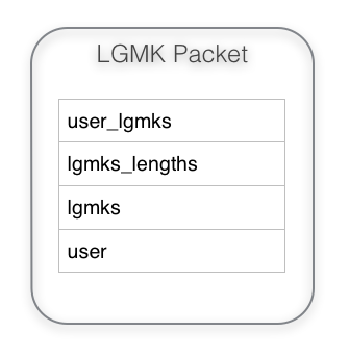
\includegraphics[keepaspectratio=true,scale=0.8]{figuras/lgmks.eps}
	\caption{Formato do pacote LGMK.}
	\label{lgmk}
\end{figure}

O campo referente ao \textbf{user\_lgmks} é um array que armazena todas as marcações fornecidas pelo usuário e seu tamanho é ilimitado. O \textbf{lgmks\_lengths} é um array responsável por armazenar o tamanho de cada marcação. A quantidade de marcações contidas no campo user\_lgmks é armazenada no \textbf{lgmks}. Por último, o campo \textbf{user} contém informações sobre o usuário que fez as marcações. Uma nova estrutura foi definida e inserida dentro do formato sem, obviamente, corrompê-lo. Foi possível codificar e também decodificar as marcações de conteúdo com integridade.

Os três \textit{header packets} definidos pelo Vorbis devem seguir a ordem disposta na Figura \ref{newformat} ou o arquivo será corrompido. O pacote LGMK não é reconhecido pelo Vorbis pelos seguintes motivos:

\begin{enumerate}
	\item O pacote possui um tipo diferente dos três tipos de cabeçalhos do Vorbis, desta forma ocorre erro no processo de decodificação.
	\item A string de identificação do pacote é ``lgmks'' e o Vorbis não irá decodificar este pacote;
	\item Quando o Vorbis for decodificar o pacote de áudio, o pacote LGMK SERÁ ignorado por ser um pacote não-áudio.
\end{enumerate}

 No entanto, a decodificação não é corrompida por conta da forma que foi estruturado o pacote e do local onde foi inserido. O pacote LGMK foi construído como sendo um pacote de cabeçalho semelhante aos \textit{header packets} do \textit{codec} Vorbis. Ou seja, ele possui um byte para a identificação do tipo de pacote de cabeçalho. A diferença está nos seis bytes subsequentes, onde a string que representa a identificação do pacote é ``lgmks''. O pacote foi inserido direto no formato recipiente Ogg logo após o terceiro pacote de cabeçalho do Voribs. A Figura \ref{newformat} mostra como ficou organizado a estruturação do formato Ogg vorbis após inserção do pacote referente a marcação de conteúdo.

 \begin{figure}[ht]
	\centering
		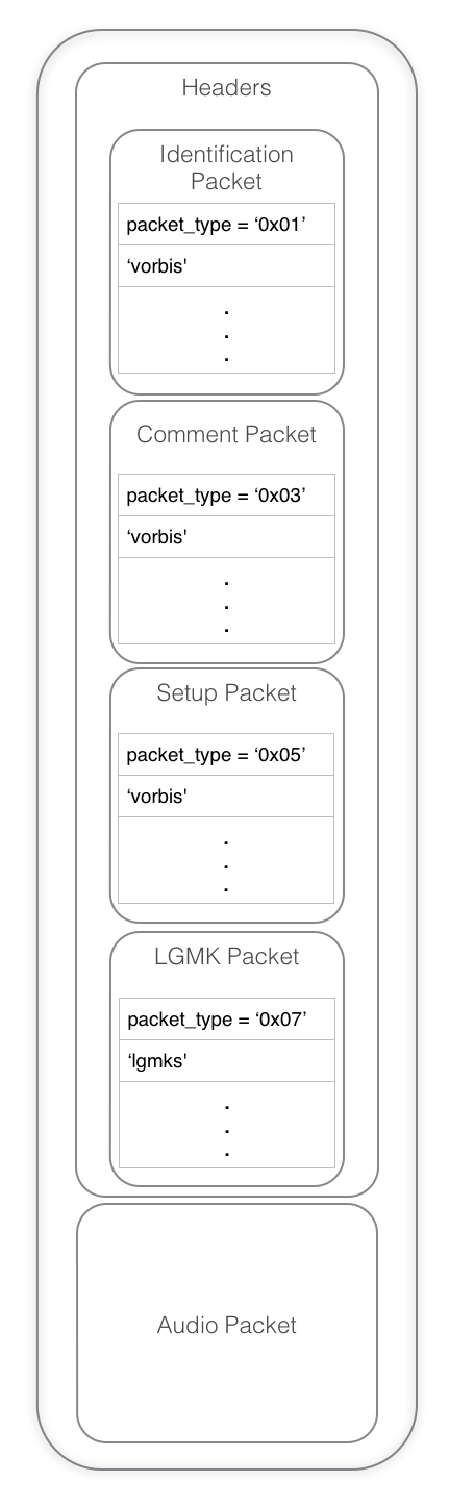
\includegraphics[keepaspectratio=true,scale=0.8]{figuras/newformat.eps}
	\caption{Estrutura Ogg Vorbis com o pacote LGMK inserido.}
	\label{newformat}
\end{figure}

Como foi posto após o cabeçalho de configuração do Ogg Vorbis, no processo de decodificação padrão, o pacote LGMK tentará ser codificado como pacote de áudio e então será ignorado. Portanto, ao executar um player o arquivo Ogg Vorbis gerado é tocado normalmente.

\section{Construção do decodificador}

Para o desenvolvimento do código referente ao processo de decodificação do arquivo *.ogg foram utilizadas as bibliotecas \textit{libvorbisfile}, \textit{libvorbis} e \textit{libogg}. A \textit{libvorbisfile} oferece o suporte necessário voltado para a decodificação do arquivo tornando o processo mais simples. Para compilar o arquivo é necessário utilizar o seguinte comando: 
	
   \$ gcc -o <nome\_para\_o\_executável> <código\_fonte> -logg -lvorbis -lvorbisfile

O código implementado decodifica os dados de cabeçalho e os imprime no terminal. Os dados PCM contidos do pacote de áudio são direcionados para um arquivo de saída.

\subsection{Decodificação dos metadados}

O metadados, uma vez codificados, precisavam ser decodificados e seu conteúdo recuperado em mémoria sem perda de dados. Para este fim, foi feito o uso da API \textit{libvorbisfile} onde foi possível recuperar os metadados corretamente.

\subsection{Decodificação do pacote LGMK}

Como dito, o pacote é inserido diretamente no contêiner Ogg, ou seja, em nenhum momento é feito uso da estrutura vorbis para a inserção do pacote. Para o processo de decodificação do pacote LGMK, e por não fazer parte da estrutura Vorbis, a biblioteca \textit{libvorbisfile} não oferece nenhum suporte e foi desconsiderada no processo de decodificação a partir deste ponto do projeto. Para alcançar o objetivo de decodificação, o uso das bibliotecas \textit{libvorbis} e \textit{logg} foram ainda mais efetivos. A \textit{libvorbis} ainda foi utilizada para decodificar a estrutura Vorbis, porém de uma forma mais ``manual''. Para o pacote LGMK foi utilizada apenas a biblioteca \textit{logg}. Ao final, todo o arquivo foi decodificado corretamente.